\documentclass[export,border=0pt]{standalone}
\usepackage[T1]{fontenc}
\usepackage{amsmath,amsfonts}
\usepackage{grid-guide}
\usepackage{tikz,pgfplots}
\usetikzlibrary{shapes.geometric} % Cylinder
\usetikzlibrary{shadows.blur,arrows.meta,bending,positioning}
\usetikzlibrary{%
	calc,%
	decorations.pathmorphing,%
	fadings,%
	shadings,
   decorations.pathreplacing,calligraphy
}
\usepackage{animate}

\begin{document}
\begin{animateinline}[loop]{1}
    \multiframe{60}{i=0+1}{
  \begin{tikzpicture}[remember picture]
    \node[anchor=center,opacity=0.5](i1) at (10,3.5){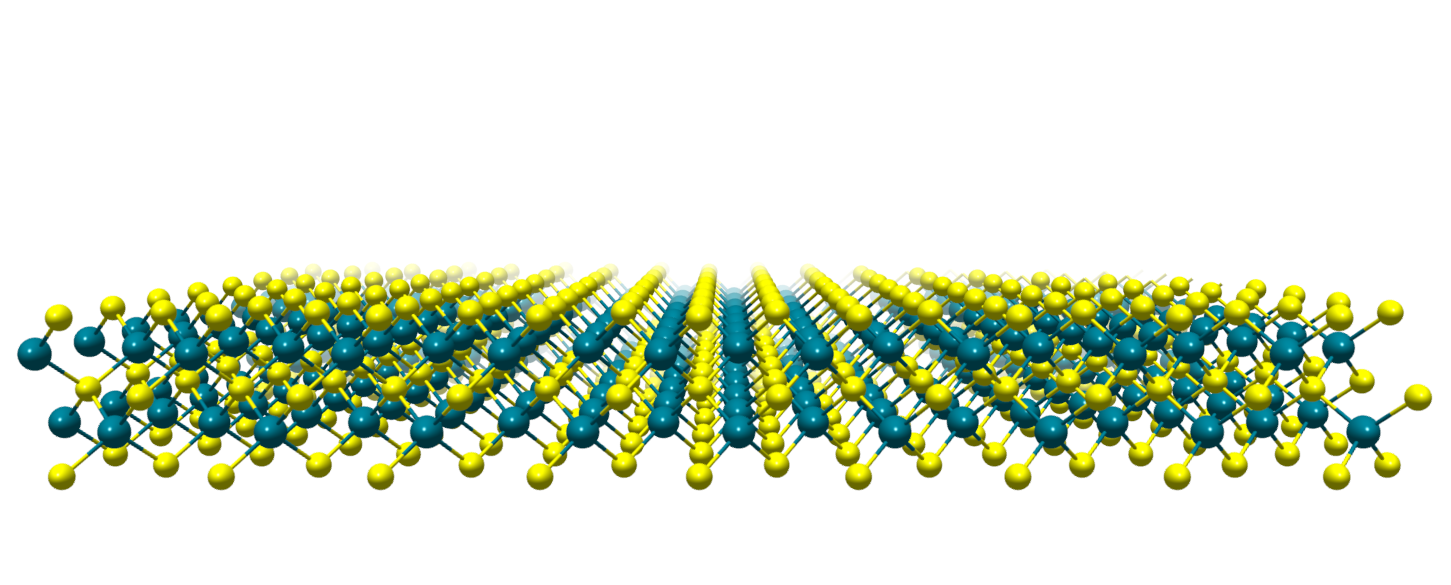
\includegraphics[width=\paperwidth]{atom-line.png}};
    %  \draw[labeled grid](0,0) to (20,7);   
    \begin{scope}[yshift=1cm,xshift=1cm]
        % \def\x{\i}
        % \def\xmax{\i}
        % \pgfmathsetmacro\xx{\i*0.2};
        % \draw[variable=x,color=red]plot[samples=100,domain=0:10] function {\i*sin(x)};
        \begin{axis}[width=18cm,height=4.5cm,hide axis,xmax=0,xmax=6*pi,ymin=-3.2,ymax=3.2]
         
          \pgfmathsetmacro\xx{\i*0.1};
          \ifnum\i<15
              \addplot[domain=0:6*pi,samples=100,line width=2pt,red] {0.2*\i*cos(deg(x))};
          \else
              \ifnum\i<30
                \addplot[domain=0:6*pi,samples=100,line width=2pt,red] {0.2*(15-(\i-15))*cos(deg(x))};
              \else
                  \ifnum\i<45
                  \addplot[domain=0:6*pi,samples=100,line width=2pt,red] {0.2*(\i-45)*sin(deg(x))};
                  \else 
                  \addplot[domain=0:6*pi,samples=100,line width=2pt,red] {0.2*(45-\i)*sin(deg(x))};
                  \fi
              \fi
          \fi
      
        \end{axis}
    \end{scope}
        
   \node[red, scale=3,anchor=north west] at (i1.north west){$\psi(\mathbf{r})=e^{i\mathbf{k}\cdot \mathbf{r}}U(\mathbf{r})$};
  \end{tikzpicture}
  }
\end{animateinline}
\end{document} 
% \draw[ultra thick, red] (0,2) sin (3,4)cos(6,2) sin (9,0) cos(12,2)sin (15,4)cos (18,2);
